\documentclass{article}
\usepackage[utf8]{inputenc}
\usepackage{amsmath}
\usepackage{listings}
\usepackage{graphicx}
\usepackage{hyperref}
\usepackage[numbers]{natbib}
\usepackage[margin=1in]{geometry}
\usepackage{titling}
\setlength{\droptitle}{-3em}
\graphicspath{ {./images/} }


\title{Real or Fake? Detecting Deepfakes}
\author{Justin Hollister}
\date{March 2026}

\begin{document}

\maketitle
\vspace{-1em}

If you have spent time on social media in the last few months you have almost certainly encountered a variety of AI generated images and videos.  Maybe you've seen a video of your English teacher dunking on Lebron \footnote{https://www.tiktok.com/@ikrrrrbwi81alt/video/7598717828409068855}, or perhaps an altered image posted by our White House\footnote{https://www.theguardian.com/us-news/2026/jan/22/white-house-ice-protest-arrest-altered-image}. With apps like Viggle Ai\footnote{It took <5 min to make a deepfake. I used an animated character but this could just as easily have been a person https://viggle.ai/share/436f2b0d-14e5-4705-9ea4-2078e33d2c76 } it is easier than ever to create and promote deepfaked images and videos of people. While these videos, when clearly false, can be very amusing, they are also capable of great societal harm. In this paper I explore and compare a few methods of detecting deepfakes via techniques covered in CS109: Naive Bayes and Logistic Regression, training and testing on the FaceForensics++~\cite{rossler2019faceforensics} benchmark dataset.

\subsection*{Qualities of a Deepfake}
Deepfaked videos, while difficult to spot with the human eye, often leave traces that computers can pick up on. FaceSwap works by detecting the face in each frame, independently estimating a warp, synthesizing a new face, and blending it onto the background. This pipeline introduces three categories of artifact: the face region is re-encoded separately from the background (leaving different compression fingerprints), the per-frame warp introduces small jitter across frames that a real face would not have, and the blending step applies sharpening that makes the face region abnormally crisp relative to the unmodified background. For every video I extracted 5 features targeting these differences (see Appendix~\ref{app:features} for full details), trained on 320 videos (200 real, 200 FaceSwap c0 from FaceForensics++\cite{rossler2019faceforensics}) and tested on 80, using a stratified video-level 80/20 split so that frames from the same video never appear in both sets.

\subsection*{Naive Bayes}
Naive Bayes was a natural first choice for this problem: my dataset is small (320 training videos), the algorithm is interpretable, and each feature captures a distinct artifact type --- compression differences, sharpness, temporal jitter --- so the independence assumption is at least defensible. The classifier works by choosing the label $y$ that maximises $P(Y = y \mid X = x)$, breaking the joint likelihood into a product of per-feature terms (one distribution per feature per class) and comparing them in log-space. See Appendix~\ref{app:derivations} for the full derivation.\footnote{Throughout, $y \in \{0, 1\}$: 0 = real, 1 = deepfake.}

The central question is how to estimate each per-feature, per-class distribution --- that is where MLE and KDE come in.

\subsubsection*{Maximum Likelihood Estimation}

MLE chooses the distribution parameters $\hat\theta$ that make the observed training data most probable, applied separately to each feature for each class. See Appendix~\ref{app:derivations} for the derivation.

The first decision is which distribution family to assume. All five features are non-negative and right-skewed, so I evaluated two options. I started with a \textbf{Gaussian} --- the simplest and most common choice --- but a Gaussian assigns probability mass to negative values and tends to underestimate the heavy tail. I therefore also tried a \textbf{Gamma} distribution, which is supported on $(0, \infty)$ and naturally handles right-skewed data. For the Gaussian, MLE yields the sample mean and variance in closed form; for the Gamma there is no closed-form solution so I used \verb|scipy.stats.gamma.fit| instead. As Figure~\ref{fig:gamma_vs_guassian_visualized} shows, neither family fits the actual distributions particularly well --- which motivated the approach below.

\subsubsection*{Kernel Density Estimation}
Since neither parametric family fit the data well, I turned to Kernel Density Estimation (KDE)\footnote{https://faculty.washington.edu/yenchic/17Sp\_403/Lec7-density.pdf} --- a non-parametric density estimator that makes no assumption about the underlying distribution. Instead of fitting parameters to a fixed family, KDE places a small symmetric bump function (\textit{kernel}) at each training point and sums them into a smooth density estimate:\footnote{KDE does not change how Naive Bayes works nor its independence assumption --- it only changes how we estimate $P(X_i = x_i \mid Y = y)$.}

\begin{equation}
\hat{f}_h(x) = \frac{1}{nh} \sum_{i=1}^n K\!\left(\frac{x - x_i}{h}\right)
\end{equation}

where $K$ is a Gaussian kernel and $h$ is the bandwidth, set automatically via Scott's rule ($h = n^{-1/5}\hat{\sigma}$)\footnote{Too small an $h$ leads to an overfit, noisy estimate; too large and it is oversmoothed. Scott's rule balances these extremes without manual tuning.}. The resulting density estimate $\hat{f}_h(x)$ is plugged directly into the Naive Bayes log-likelihood in place of the parametric PDF. See Appendix~\ref{app:derivations} for the full kernel and bandwidth details.

\subsection*{Logistic Regression}
After running Naive Bayes I wanted to see whether relaxing the independence assumption would help. My five features all capture compression and sharpness artifacts, so they are inevitably correlated --- Naive Bayes double-counts that shared evidence every time a new feature is added. Logistic regression learns a single linear decision boundary directly over all features jointly, avoiding this problem entirely. It assumes the outcome is Bernoulli and maximises the resulting log-likelihood via gradient descent; since no closed-form solution exists, weights are estimated numerically. See Appendix~\ref{app:derivations} for the full derivation.

\subsubsection*{Youden's J Threshold}
All four methods output a probability $P(\text{fake} \mid X = x)$, and I applied a shared threshold-calibration step to each. When a model's scores are systematically biased toward one end of $[0, 1]$, a fixed 0.5 cutoff misclassifies borderline cases that the scores' own natural separation could resolve --- in practice I found this left meaningful accuracy on the table. Rather than a full calibration procedure like Platt's scaling\footnote{Platt scaling fits a sigmoid to the raw output scores on a held-out calibration set.}, I used Youden's J Statistic\footnote{Youden, W.J. (1950). Index for rating diagnostic tests. \textit{Cancer}, 3(1), 32--35.}: sweep every candidate threshold on the training scores and pick the one that maximises

\begin{equation}
J = \text{TPR} - \text{FPR}
\end{equation}

Geometrically, this is the point on the ROC curve furthest from the diagonal of no-discrimination. The threshold found on the training set is then applied as-is at test time. See Appendix~\ref{app:derivations} for full definitions.

\subsection*{Results}

  \begin{table}[h]
  \centering
  \begin{tabular}{lcccc}
  \hline
  & \multicolumn{2}{c}{\textbf{f5 only}} & \multicolumn{2}{c}{\textbf{All 5 features}} \\
  \textbf{Method} & \textbf{Acc} & \textbf{AUC} & \textbf{Acc} & \textbf{AUC} \\
  \hline
  KDE-NB        & \textbf{0.688} & 0.683 & 0.637 & 0.670 \\
  Logistic Reg. & 0.588 & 0.680 & \textbf{0.688} & \textbf{0.720} \\
  Gaussian NB   & 0.588 & 0.680 & 0.600 & 0.666 \\
  Gamma NB      & 0.588 & 0.671 & 0.588 & 0.655 \\
  \hline
  Majority class & 0.500 & 0.500 & 0.500 & 0.500 \\
  Random         & $\approx$0.500 & $\approx$0.500 & $\approx$0.500 & $\approx$0.500 \\
  \hline
  \end{tabular}
  \caption{Accuracy and AUC\protect\footnote{AUC (Area Under the ROC Curve) measures ranking ability --- the probability the model scores a fake higher than a real --- independently of any threshold. \textit{Majority class} always predicts ``fake''; \textit{Random} flips a fair coin. See Appendix~\ref{app:figures} for confusion matrices and ROC curves.} on 80 test videos (320 train), split evenly between real and fake.}
  \label{tab:results}
  \end{table}

I tested each method on two feature configurations: f5 alone --- our strongest individual feature\footnote{f5 is the Laplacian variance ratio, the variance of the Laplacian filter response in the face region divided by that of the background. See Appendix~\ref{app:features} for the full derivation.} --- and all 5 together. For f5-only, KDE-NB leads on both accuracy (0.688) and AUC (0.683), modestly outperforming Gaussian NB (0.680) and Gamma NB (0.671). The AUC gap is small, suggesting the large accuracy difference (0.688 vs.\ 0.588) is driven primarily by better probability calibration rather than improved class separation.\footnote{AUC measures ranking ability independently of any threshold. Because KDE fits the actual density shape more faithfully, it pushes fake scores closer to 1 and real scores closer to 0, so the Youden's J threshold lands in a cleaner spot --- yielding higher accuracy without requiring a meaningfully better ranking.}

With all 5 features the picture flips: Logistic Regression takes the top spot (0.688 accuracy, 0.720 AUC) while KDE-NB drops by 0.051. The NB independence assumption is heavily violated --- our features are correlated, so each additional feature double-counts evidence and inflates the false positive rate (see Figure~\ref{fig:confusion_matrices_all_methods}). Logistic regression avoids this by learning a single linear decision boundary over all features rather than multiplying independent likelihoods. With only one feature, Logistic Regression and Gaussian NB produce identical scores (0.588 accuracy, 0.680 AUC) --- both are outperformed by KDE-NB, which achieves 0.688 accuracy on the same feature. This confirms that with a single feature the bottleneck is density estimation quality, not the classifier form. Overall I give the edge to logistic regression: its 0.037 AUC advantage suggests stronger ranking ability that would likely widen on a larger test set.


\subsection*{The Future of Deepfake Detection}
The best result we were able to achieve was an accuracy of 68.8 percent, meaning we still misidentify over 30 percent of videos. Our model did not treat a false positive or false negative differently, though one might argue that in the field of deepfake detection a false negative, falsely classifying a deepfaked video as real, to be much more harmful. Modern deepfake detection systems generally use deep learning to achieve accuracies above 99 percent on benchmarks like FF++ --- substantially better than our 68.8\%. Most of these deep learning models operate directly on pixels (or a combination) rather than through predefined features like ours, which requires significantly more training data. I trained my model on 320 videos (200 deepfakes and 200 real total, 80/20 train/test split) and tested on 80 videos of an even split. For reference FF++ has 5000 videos total, and other datasets have far more. My model is far from effective, but it was a genuinely interesting exercise in probabilistic classifiers.

\subsection*{LLM Usage}
I used LLMs, specifically Claude Code's Sonnet 4.6, to help me program much of first version of the code. All of the feature extraction code is done by LLM, as like I mentioned in the writeup, my focus was on the classification methods, and much of the detail of each features are outside my domain of knowledge (the require in depth knowledge about image processing and compression and more). I tested dozens of variations of features, and used LLMs to quickly implement features to test and verify the accuracy before I devoted too much time into anything. I also used LLMs to generate the initial code for classification, again to verify the approach and accuracy, before going back through and rewriting functions that used libraries such as \verb|scipy| and \verb|sklearn|, with my own implementations. I also used LLM's to refine this paper (ie. check for typos, errors, shorten my argument to reach 3 pages etc.). 

\newpage
\appendix
\section{Feature Descriptions}
\label{app:features}

For every video in the dataset I extract 5 scalar features. Each feature compares a \textit{face region} to a \textit{background region} within the same frame. The face is detected with OpenCV's Haar Cascade classifier, and the bounding box is tightened by 15\% on the left and right, 10\% on the top, and 20\% on the bottom to focus on the core face and reduce hair/neck contamination. The background is the remainder of the frame after removing the (un-tightened) bounding box. Ten frames are sampled uniformly from each video, and per-frame feature values are averaged to produce a single video-level feature vector.

\subsection*{f1 — DCT Chi-Squared Divergence}

\textbf{Intuition.} FaceSwap pastes a synthetically generated face onto an unmodified background. The face region has been processed through at least one additional encode-decode cycle, so its frequency-domain content should look systematically different from the native background.

\textbf{Computation.} Both the face crop and the background region are converted to grayscale and a 2D Discrete Cosine Transform (DCT) is applied to each. The DCT expresses an image patch as a sum of cosine waves at different spatial frequencies; compression artifacts show up as anomalies in the coefficient magnitudes. We then build a 50-bin normalized histogram of the DCT coefficients for each region:

\[
  P_k = \frac{\text{count}(\text{face coefficients in bin } k)}{\text{total face coefficients}}, \quad
  Q_k = \frac{\text{count}(\text{background coefficients in bin } k)}{\text{total background coefficients}}
\]

The symmetric chi-squared divergence\footnote{The standard chi-squared divergence uses only $Q_k$ in the denominator. Using $P_k + Q_k$ makes the measure symmetric in $P$ and $Q$, which is preferable here since neither the face nor the background is a fixed reference distribution.} between these two distributions is the feature:

\[
  f_1 = \chi^2(P, Q) = \sum_{k=1}^{50} \frac{(P_k - Q_k)^2}{P_k + Q_k + \varepsilon}
\]

A log transform ($\log(1 + f_1)$) is applied at training time to correct the heavy right skew of the raw values.

\subsection*{f2 — Block-DCT $\beta$-Statistic Divergence}

\textbf{Intuition.} JPEG and video codecs compress images in $8\times 8$ pixel blocks using the DCT. When a face region is re-encoded (as happens in FaceSwap), each AC coefficient position accumulates a different amount of quantization noise than the surrounding background. This changes the \textit{scale} of the coefficient distribution at each AC position in a measurable way, even on lossless (c0) source files where the original compression is preserved.

\textbf{Computation.} The face and background regions are each divided into non-overlapping $8\times8$ pixel blocks. A 2D DCT is applied to every block. For each of the 63 AC coefficient positions (the DC component at position 0 is skipped because it simply encodes average brightness), we collect the coefficient values across all blocks and compute the scale parameter:

\[
  \beta_j = \frac{\text{std}(\{c_{b,j} : b = 1,\ldots,B\})}{\sqrt{2}}, \quad j = 1, \ldots, 63
\]

where the $\sqrt{2}$ normalisation gives the scale parameter of a zero-mean Laplace distribution\footnote{For a zero-mean Laplace distribution with scale $b$, the standard deviation is $b\sqrt{2}$, so $b = \text{std}/\sqrt{2}$. DCT AC coefficients across blocks are empirically well-approximated by a Laplace distribution, following Giudice et al.\ (2021).}, the distribution that empirically fits DCT coefficients well.

This gives two 63-dimensional vectors, $\boldsymbol{\beta}^{\text{face}}$ and $\boldsymbol{\beta}^{\text{bg}}$. The feature is the mean absolute difference across all positions:

\[
  f_2 = \frac{1}{63} \sum_{j=1}^{63} \left| \beta_j^{\text{face}} - \beta_j^{\text{bg}} \right|
\]

This approach is based on Giudice et al.\ (2021)\footnote{Giudice et al., ``Fighting Deepfakes by Detecting GAN DCT Anomalies'', \textit{MDPI Journal of Imaging}, 2021.}. A log transform is applied at training time.

\subsection*{f3 — Absolute Difference of Mean Absolute DCT Coefficients}

\textbf{Intuition.} AI face synthesis often introduces a slight blurring or smoothing of the face relative to the original. In the frequency domain, blurring suppresses high-frequency coefficients, reducing the average coefficient magnitude. If the face is blurrier than the background we expect the mean absolute DCT coefficient to be lower for the face than for the background.

\textbf{Computation.} Full-image 2D DCTs are applied to the grayscale face and background patches. The mean of the absolute values of all coefficients is computed for each:

\[
  \mu_{\text{face}} = \frac{1}{MN}\sum_{u,v} |F_{\text{face}}[u,v]|, \quad
  \mu_{\text{bg}} = \frac{1}{M'N'}\sum_{u,v} |F_{\text{bg}}[u,v]|
\]

The feature is:

\[
  f_3 = |\mu_{\text{face}} - \mu_{\text{bg}}|
\]

A log transform is applied at training time.

\subsection*{f4 — Frame-to-Frame Temporal Inconsistency}

\textbf{Intuition.} FaceSwap estimates the warp for each frame independently, which introduces small jitter in the pasted face from one frame to the next that does not follow the smooth natural motion of a real face. We should therefore see higher frame-to-frame pixel variation in the face region of deepfakes than in real videos.

\textbf{Computation.} Consecutive pairs of sampled frames $(t, t+1)$ are used. Each face crop is resized to $64\times64$, converted to grayscale, and mean-normalized to remove global lighting drift:

\[
  \tilde{I}_t = \frac{I_t}{\text{mean}(I_t) + \varepsilon}
\]

The Mean Absolute Deviation (MAD) between consecutive normalized crops is computed, then averaged across all pairs:

\[
  f_4 = \frac{1}{T-1} \sum_{t=1}^{T-1} \frac{1}{64^2}\sum_{i,j}\left|\tilde{I}_t[i,j] - \tilde{I}_{t+1}[i,j]\right|
\]

where $T = 10$ is the number of sampled frames. No log transform is applied to $f_4$.

\subsection*{f5 — Laplacian Variance Ratio}

\textbf{Intuition.} FaceSwap applies a blending and sharpening step when compositing the generated face onto the background frame. This introduces ringing and edge-enhancement artifacts in the face region that raise its apparent sharpness above that of the surrounding (unmodified) background. The Laplacian filter is the standard tool for measuring image sharpness, since it amplifies rapid intensity changes (edges, texture, ringing).

\textbf{Computation.} The discrete Laplacian operator $\nabla^2$ is applied to the grayscale face and background:

\[
  \nabla^2 f[i,j] = f[i+1,j] + f[i-1,j] + f[i,j+1] + f[i,j-1] - 4f[i,j]
\]

The feature is the ratio of their variances:

\[
  f_5 = \frac{\text{Var}(\nabla^2 I_{\text{face}})}{\text{Var}(\nabla^2 I_{\text{bg}}) + \varepsilon}
\]

Higher $f_5$ means the face is sharper (or more artifact-laden) relative to the background. A log transform is applied at training time. $f_5$ was by far the strongest individual discriminator, achieving the best standalone AUC (0.683) of all five features.

\newpage
\section{Figures}
\label{app:figures}

\begin{figure}[h]
    \centering
    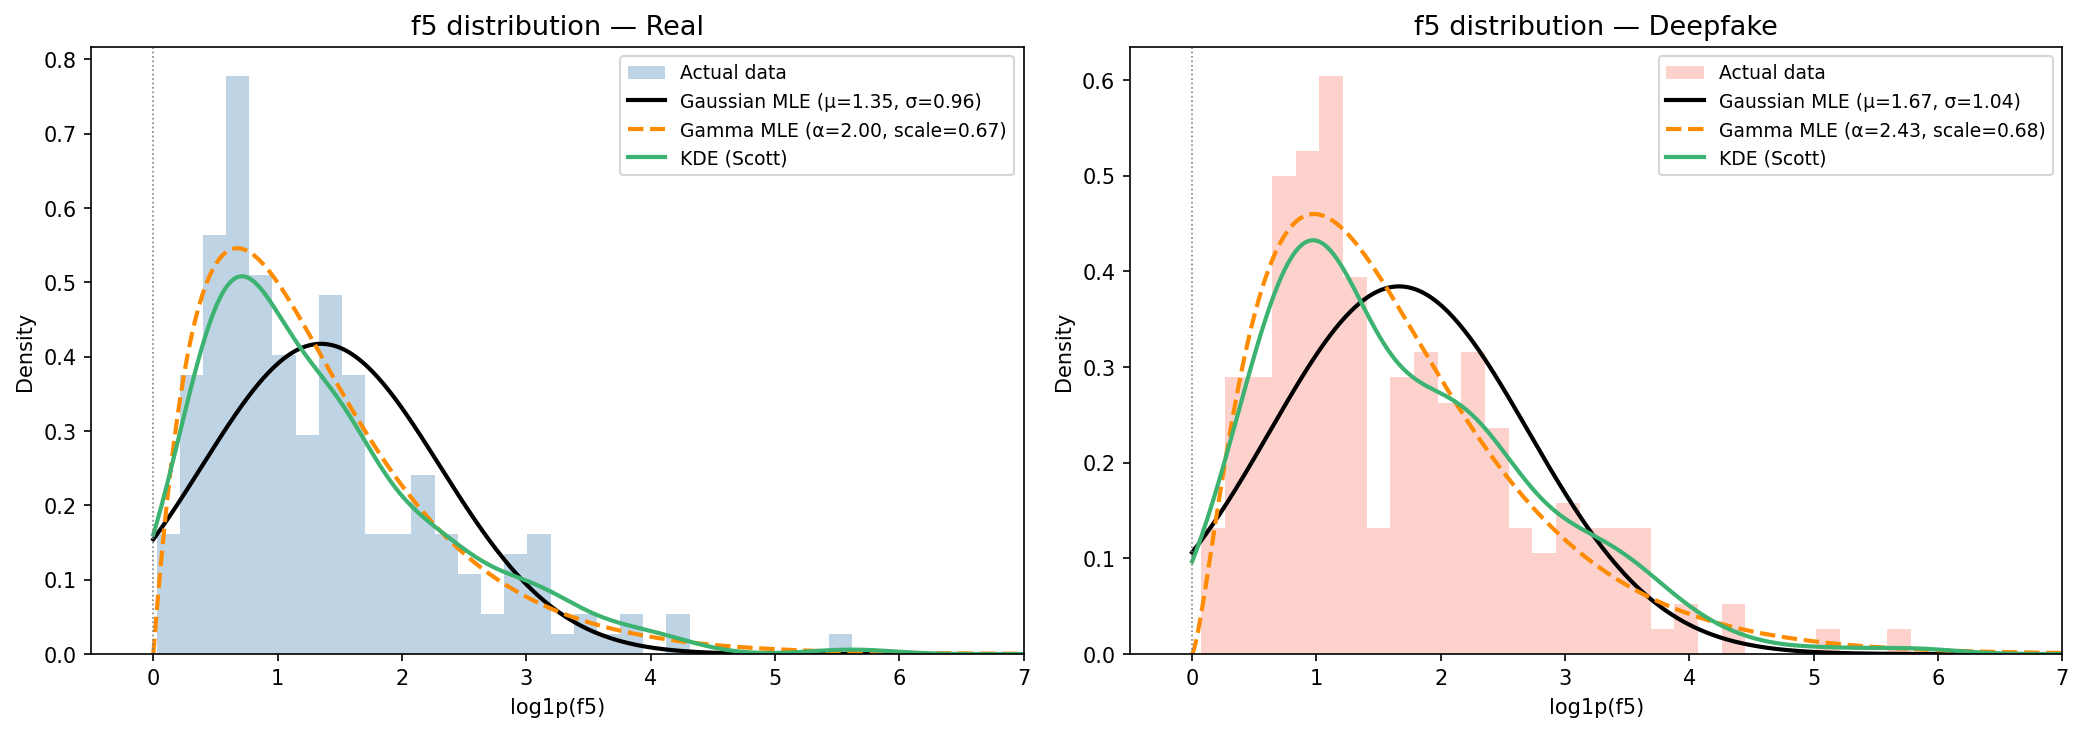
\includegraphics[width=0.9\linewidth]{images/f5_distribution_all_fits.png}
    \caption{Distribution of the f5 feature (Laplacian variance ratio) for real and deepfaked videos, with Gaussian, Gamma, and KDE fits overlaid. KDE most closely matches the actual data shape, motivating its use over parametric MLE.}
    \label{fig:gamma_vs_guassian_visualized}
\end{figure}

\begin{figure}[h]
    \centering
    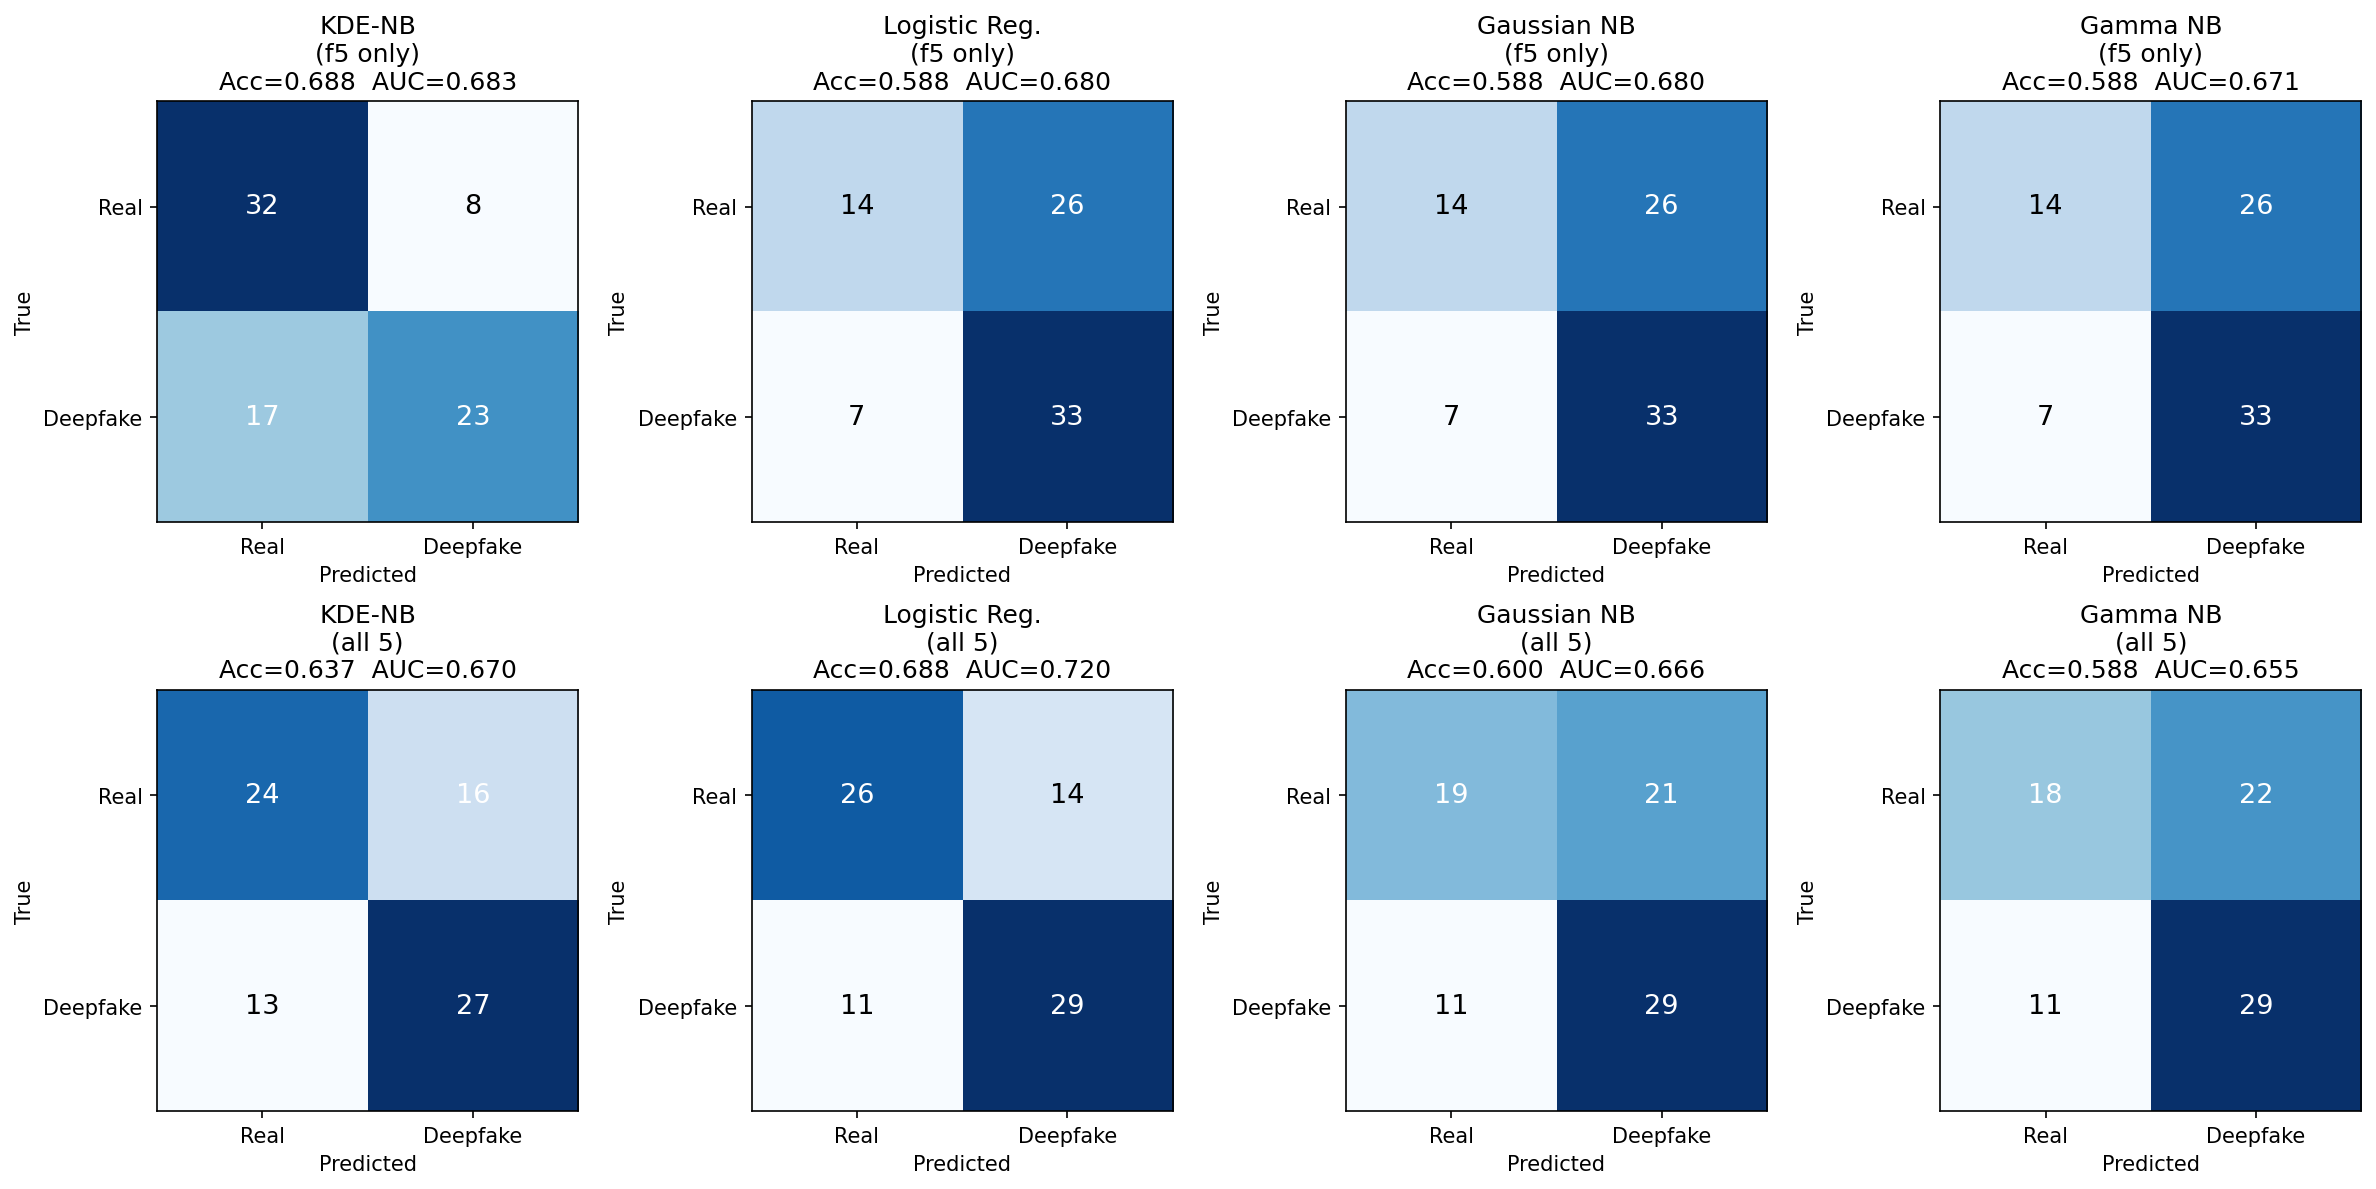
\includegraphics[width=0.75\linewidth]{images/confusion_matrices_all_methods.png}
    \caption{Confusion matrices for all methods (rows: f5-only and all-5-features configurations). Each cell shows the count out of 80 test videos. Note the higher false-positive rate when KDE-NB uses all five features, consistent with the NB independence assumption being violated.}
    \label{fig:confusion_matrices_all_methods}
\end{figure}

\begin{figure}[h]
    \centering
    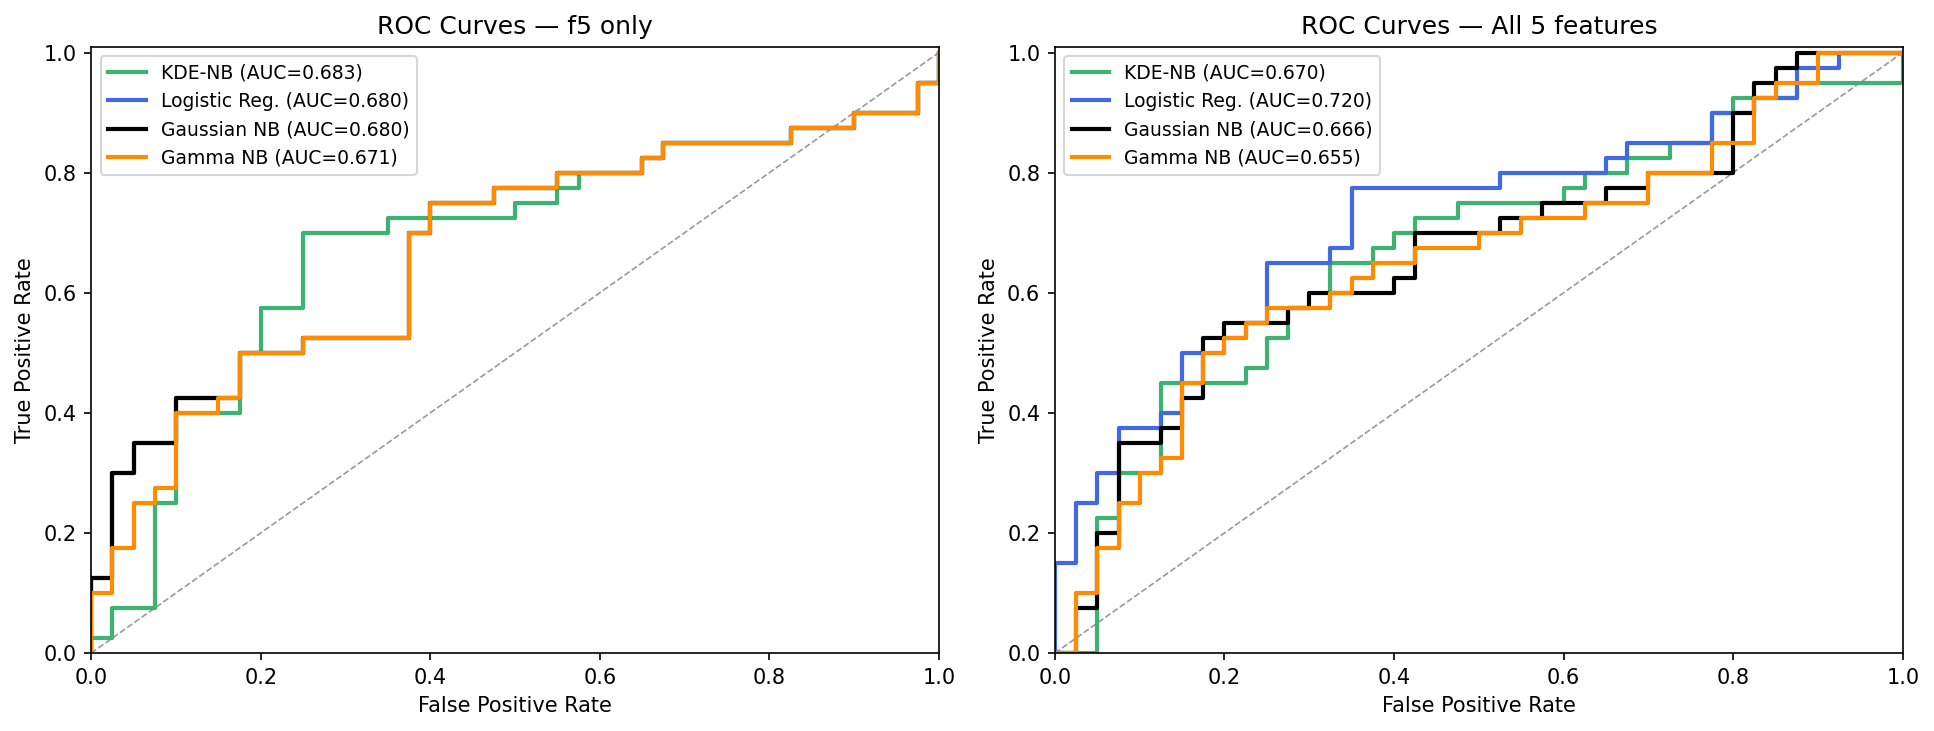
\includegraphics[width=0.85\linewidth]{images/roc_comparison_all_methods.png}
    \caption{ROC curves for all methods and feature configurations. The diagonal dashed line represents random chance (AUC = 0.500). Logistic Regression with all five features achieves the highest AUC (0.720), while all methods substantially outperform the random baseline regardless of feature set.}
    \label{fig:roc_all_methods}
\end{figure}

\begin{figure}[h]
    \centering
    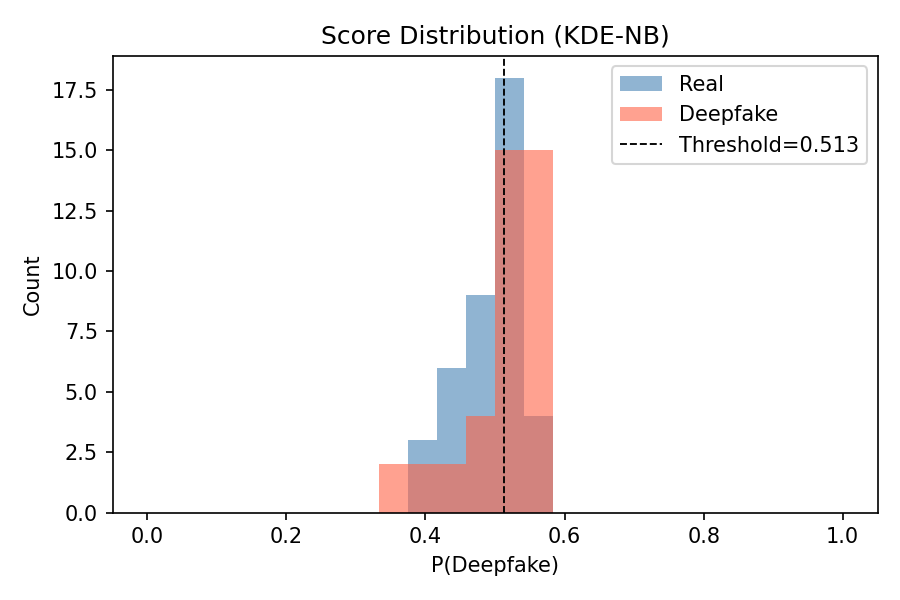
\includegraphics[width=0.75\linewidth]{images/score_distribution_f5.png}
    \caption{Posterior score distributions ($P(\text{fake} \mid \mathbf{x})$) for the KDE-NB classifier using f5 only. Real videos (blue) are concentrated near 0 and deepfakes (orange) near 1, with meaningful separation despite overlap. The vertical dashed line marks the Youden's J threshold ($\tau \approx 0.513$).}
    \label{fig:score_distribution_f5}
\end{figure}

\begin{figure}[h]
    \centering
    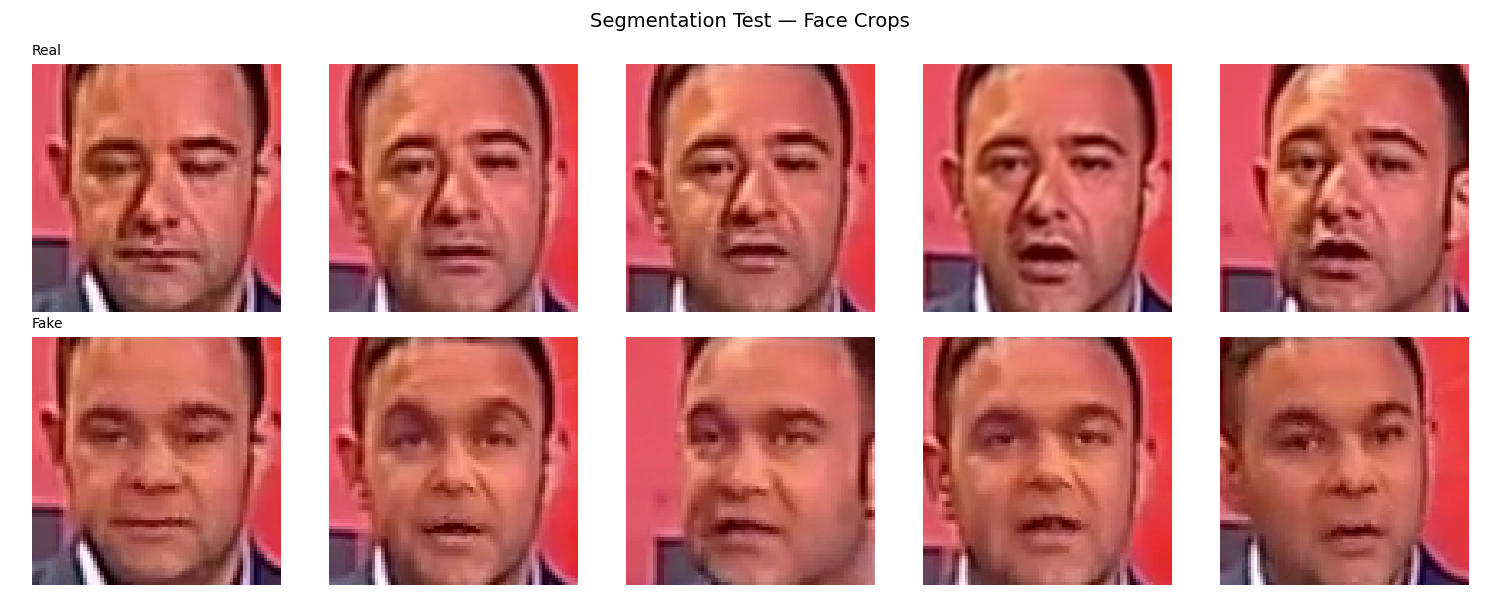
\includegraphics[width=0.75\linewidth]{images/segmentation_test.png}
    \caption{Example face segmentation output from the OpenCV Haar Cascade detector. The tighter bounding box (15\% inset left/right, 10\% top, 20\% bottom) focuses on the core face region, reducing contamination from hair and neck.}
    \label{fig:segmentation}
\end{figure}

\newpage
\section{Mathematical Derivations}
\label{app:derivations}

\subsection*{Naive Bayes Derivation}
With any classification algorithm ($y \in \{0,1\}$) we seek the label that maximises $P(Y = y \mid X = x)$:
\begin{equation}
\begin{aligned}
\hat y &= \text{arg max} \ P(Y = y | X = x) \\
&= \text{arg max} \ \frac{P(Y = y)P(X = x | Y = y)}{P(X = x)} \\
&= \text{arg max} \ P(Y = y)P(X = x | Y = y) \quad \text{(since $P(X=x)$ is constant w.r.t.\ $Y$)}
\end{aligned}
\end{equation}
Naive Bayes assumes each feature $x_i$ is independent of the others given $y$, factorising the joint likelihood into a product of per-feature terms:
\begin{equation}
\begin{aligned}
\hat y &= \text{arg max} \ P(Y = y)\prod_i P(X_i = x_i | Y = y) \\
&= \text{arg max} \ \log P(Y = y) + \sum_i \log P(X_i = x_i | Y = y)
\end{aligned}
\end{equation}

\subsection*{Normal MLE Estimation}
A Gaussian has two parameters: $\mu = \theta_0$ and $\sigma^2 = \theta_1$.
\begin{equation}
\begin{aligned}
L(\theta) &= \prod_{i=1}^n f(X_i|\theta)
= \prod_{i=1}^n \frac{1}{\sqrt{2\pi\theta_1}}e^{-\frac{(x_i-\theta_0)^2}{2\theta_1}} \\
LL(\theta) &= -\frac{n}{2}\log(2\pi\theta_1) - \frac{1}{2\theta_1}\sum_{i=1}^n(x_i - \theta_0)^2 \\
\frac{\partial LL}{\partial \theta_0} = 0 &\implies \hat{\theta}_0 = \frac{1}{n}\sum_{i=1}^n x_i = \bar{x} \\
\frac{\partial LL}{\partial \theta_1} = 0 &\implies \hat{\theta}_1 = \frac{1}{n}\sum_{i=1}^n(x_i - \bar{x})^2
\end{aligned}
\end{equation}

\subsection*{Gamma MLE Estimation}
A Gamma distribution has two parameters: $\alpha = \theta_0$ (shape) and $\beta = \theta_1$ (scale).
\begin{equation}
\begin{aligned}
L(\theta) &= \prod_{i=1}^n \frac{1}{\Gamma(\theta_0)\theta_1^{\theta_0}} x_i^{\theta_0-1} e^{-x_i/\theta_1} \\
LL(\theta) &= -n\log\Gamma(\theta_0) - n\theta_0\log\theta_1 + (\theta_0-1)\sum_{i=1}^n\log x_i - \frac{1}{\theta_1}\sum_{i=1}^n x_i
\end{aligned}
\end{equation}
There is no closed-form solution; parameters are estimated numerically via \verb|scipy.stats.gamma.fit|.

\subsection*{Kernel Density Estimation --- Gaussian Kernel and Scott's Rule}
The Gaussian kernel used in equation (7) of the main text is:
\begin{equation}
K(u) = \frac{1}{\sqrt{2\pi}} e^{-u^2/2}
\end{equation}
Scott's rule selects the bandwidth automatically:
\begin{equation}
h = n^{-1/5} \hat{\sigma}
\end{equation}
where $\hat{\sigma}$ is the sample standard deviation. Too small an $h$ leads to an overfit, noisy estimate; too large and the estimate is oversmoothed.

\subsection*{Logistic Regression --- Bernoulli MLE}
Assuming $Y \sim \text{Bern}(\sigma(\theta^T \mathbf{x}))$, the likelihood and log-likelihood are:
\begin{equation}
\begin{aligned}
L(\theta) &= \prod_{i=1}^n \sigma(\theta^T \mathbf{x}^{(i)})^{y^{(i)}} \cdot \left[1 - \sigma(\theta^T \mathbf{x}^{(i)})\right]^{(1-y^{(i)})} \\
LL(\theta) &= \sum_{i=1}^n y^{(i)} \log \sigma(\theta^T \mathbf{x}^{(i)}) + (1 - y^{(i)}) \log\left[1 - \sigma(\theta^T \mathbf{x}^{(i)})\right]
\end{aligned}
\end{equation}
Parameters are found by gradient descent: $\theta \leftarrow \theta - \alpha \nabla_\theta (-LL(\theta))$.

\subsection*{Youden's J --- Full Definitions and Threshold Selection}
TPR (True Positive Rate) and FPR (False Positive Rate) are defined as:
\begin{equation}
\text{TPR} = \frac{TP}{TP + FN} \qquad \text{FPR} = \frac{FP}{FP + TN}
\end{equation}
The optimal threshold is:
\begin{equation}
\hat{\tau} = \underset{\tau}{\text{arg max}} \ J(\tau) = \underset{\tau}{\text{arg max}} \ [\text{TPR}(\tau) - \text{FPR}(\tau)]
\end{equation}
Geometrically, this corresponds to finding the point on the ROC curve that is furthest from the diagonal line of no-discrimination, maximizing the gap between model performance and random chance.

\bibliographystyle{plainnat}
\bibliography{references}

\end{document}

